\documentclass[sigconf]{acmart}

\fancyhf{} % Remove fancy page headers 
% \fancyhead[C]{Anonymous submission \#9999 to ACM CCS 2017} % TODO: replace 9999 with your paper number
\fancyfoot[C]{\thepage}

\setcopyright{none} % No copyright notice required for submissions
% \acmConference[Anonymous Submission to ACM CCS 2017]{ACM Conference on Computer and Communications Security}{Due 19 May 2017}{Dallas, Texas}
% \acmYear{2017}

\settopmatter{printacmref=false, printccs=true, printfolios=true} % We want page numbers on submissions

%%\ccsPaper{9999} % TODO: replace with your paper number once obtained
\usepackage{amsmath,amsfonts,amssymb,amsthm,epsfig,epstopdf,titling,url,array}
\newcommand{\bysinfer}{\mathsf{BI}}
\newcommand{\hlg}{\mathsf{H}}
\newcommand{\betafun}{\mathsf{beta}}
%\newcommand{\theHalgorithm}{\arabic{algorithm}}
\theoremstyle{plain}
\newtheorem{thm}{Theorem}[section]
\newtheorem{lem}[thm]{Lemma}
\newtheorem{prop}[thm]{Proposition}
\newtheorem*{cor}{Corollary}

\theoremstyle{definition}
\newtheorem{defn}{Definition}[section]
\newtheorem{conj}{Conjecture}[section]
\newtheorem{exmp}{Example}[section]

\theoremstyle{remark}
\newtheorem*{rem}{Remark}
\newtheorem*{note}{Note}

\usepackage{accents}

\begin{document}
\title{Accuracy Analysis For Three Mechanisms}


\begin{abstract} 
\end{abstract}


\keywords{Accuracy analysis} % TODO: replace with your keywords

\maketitle

\section{Introduction}
\label{sec_intro}


\section{Algorithm Setting up}
\label{sec_setup}
Given a prior distribution $\bprior=\betad(\alpha, \beta)$ and a sequence of $n$ observations $\dataobs\in\{0,1\}^n$, we define the follwing set:

\[
  \candidateset\equiv\{\betad(\alpha',\beta')\mid \alpha'=\alpha+\Delta\alpha, \beta'=\beta+n-\Delta\alpha\}
\]

where $\Delta\alpha$ is as defined in Section
\ref{sec_background}. Notice that $\candidateset$ has $n + 1$ elements, and
the Bayesian Inference process will produce an element from $\candidateset$
that we denote by $\bysinfer(\dataobs)$ -- we don't explicitely
parametrize the result by the prior, which from now on we consider
fixed and we denote it by $\bprior$.

\subsection{Baseline Approaches} 


\subsubsection{Exponential Mechanism}

Exponential mechanism $\expmech{}{x}{u}{\candidateset}$ samples a element from the candidate set $\candidateset = \{r_1, r_2, \cdots r_n\}$ with probability proportional to $exp(\frac{\epsilon u(x,r)}{2 GS})$:
\begin{equation*}
\underset{z \thicksim \expmech{}{x}{u}{\candidateset} }{Pr}[z=r] = \frac
{exp(\frac{\epsilon u(x,r)}{2 GS})}
{\Sigma_{r' \in \mathcal{R}}\ exp(\frac{\epsilon u(x,r')}{2 GS})},
\end{equation*}
where $u(x,r)$ is the Hellinger scoring function over candidates, $\hellinger(\bysinfer(\dataobs), r)$, and $GS(x)$ is the global sensitivity calculated by:
\begin{equation*}
GS = 
\max_{\{|\dataobs,\dataobs'| \leq 1;\dataobs,\dataobs'\in \mathcal{X}^n\}}\max_{\{r\in \mathcal{R}\}}
|\hellinger(\bysinfer(\dataobs), r) - \hellinger(\bysinfer(\dataobs'), r)|
\end{equation*}

Exponential mechanism is $\epsilon -$differential privacy\cite{dwork2014algorithmic}.


\subsubsection{Exponential Mechanism with Local Sensitivity}
\label{subsec_emls}
% \subsubsection{Mechanism Set up}
Exponential mechanism with local sensitivity $\expmech{local}{x}{u}{\candidateset}$ share the same candidate set and utility function as it with global sensitivity. This outputs a candidate $r \in \mathcal{R}$ with probability proportional to $exp(\frac{\epsilon u(x,r)}{2 LS(x)})$:
\begin{equation*}
\underset{z \thicksim \expmech{local}{x}{u}{\candidateset}}{\Pr}[z=r] = \frac
{exp(\frac{\epsilon u(x,r)}{2 LS(x)})}
{\Sigma_{r' \in \mathcal{R}}\ exp(\frac{\epsilon u(x,r')}{2 LS(x)})},
\end{equation*}

where local sensitivity is calculated by:

\begin{equation*}
LS(\dataobs)=\max_{\dataobs' \in \datauni^n:\adj{\dataobs}{\dataobs'}, r\in \mathcal{R}}\lvert \hellinger(\bysinfer(\dataobs'), r) - \hellinger(\bysinfer(\dataobs'), r)\rvert.
\end{equation*}

The exponential mechanism with local sensitivity is non-differential privacy\cite{dwork2014algorithmic}.



\subsubsection{Laplace Mechanism}
\begin{itemize}
  \item Release $\betad(\alpha +  \lfloor\widetilde{\Delta \alpha}\rfloor^n_0,\beta + n - \lfloor\widetilde{\Delta \alpha}\rfloor^n_0)$.
  \item $\widetilde{\Delta \alpha}\sim \lap{\Delta\alpha}{\frac{\Delta \bysinfer}{\epsilon}}$.
  % \item \todo{$S\propto ||\cdot ||_{1}$}.
  \item $\Delta \bysinfer \equiv \max\limits_{\dataobs, \dataobs' \in \{0,1\}^{n}, ||\dataobs - \dataobs'||_1 \leq 1} ||\bysinfer(\dataobs) - \bysinfer(\dataobs')||_1$.
  \end{itemize}



\subsubsection{Improved Baseline Approach}

y using sensitivity 1 in 2 dimensions and 2 in higher dimensions.
    Indeed: we can see the output of the Bayesian inference as a histogram, and $||\bysinfer(\dataobs)-\bysinfer(\dataobs')||_1 \leq 2$.


\subsection{Our approach: smoothed Hellinger distance based exponential mechanism}
\label{sec_smoo}

\subsubsection{Setting up}

\begin{definition}
\label{def_smoo}
The mechanism $\hexpmech(x)$ outputs a candidate $r \in \candidateset$ with probability
\begin{equation*}
\underset{z \thicksim \hexpmech}{\Pr}[z=r] = \frac {exp\big(\frac{-\epsilon\cdot\hellinger(\bysinfer(\dataobs),r)}{2\cdot S(\dataobs)}\big)}
{\displaystyle\sum_{r\in\candidateset} exp\Big(\frac{-\epsilon\cdot\hellinger(\bysinfer(\dataobs),r)}{2\cdot S(\dataobs)}\Big)}.
\end{equation*}
where $S_\beta(x)$ is the smooth sensitivity of $\hlg(\bysinfer(x),-)$, calculated by:

\begin{equation}
  \label{eq:smooth}
   S(\dataobs)=\max_{\dataobs' \in \{0,1\}^{n}}\bigg \{LS(\dataobs') \cdot e^{-\gamma\cdot d(\dataobs,\dataobs')}\bigg\},
\end{equation}
where $d$ is the Hamming distance between two datasets, and $\beta =
\beta(\epsilon, \delta)$ is a function of $\epsilon$ and $\delta$. 
\end{definition}

This mechanism is based on the basic exponential mechanism
\cite{talwar}, with $\candidateset$ as the range and
$\hellinger(\cdot,\cdot)$ as the scoring function. The difference is
that in this mechanism we don't calibrate the noise w.r.t. to the
global sensitivity of the scoring function but w.r.t. to the smooth
sensitivity $S(\dataobs)$ -- defined by \citet{nissim2007smooth}-- of
$\hellinger(\bysinfer(\dataobs), \cdot)$.

$\gamma = \gamma(\epsilon, \delta)$ is a function of $\epsilon$ and $\delta$ to
be determined later, and where $LS(\dataobs')$ denotes the local
sensitivity at $\bysinfer(\dataobs')$, or equivalently at $\dataobs'$,
of the scoring function used in our mechanism.

This mechanism also extends to the Dirichlet-Multinomial system $\dirichlet(\valpha)$ by rewriting the Hellinger distance as:
\[
  \hellinger(\dirichlet(\valpha_1), \dirichlet(\valpha_2)) = \sqrt{1 - \frac{\betaf(\frac{\valpha_1 + \valpha_2}{2})}{\sqrt{\betaf(\valpha_1) \betaf(\valpha_2)}}},
\]
and by replacing the $\candidateset$ with set of posterior Dirichlet
distributions candidates. Also, the smooth sensitivity $S(\dataobs)$
in (\ref{eq:smooth}) will be computed by letting $\dataobs'$ range
over all the elements in $\datauni^{n}$ adjacent to $\dataobs$. Notice
that $\candidateset$ has $\binom{n + 1}{m - 1}$ elements in this case. We
will denote by $\hexpmechd$ the mechanism for the
Dirichlet-Multinomial system.


By setting the $\gamma$ as $\ln(1 - \frac{\epsilon}{2 \ln (\frac{\delta}{2 (n + 1)})})$, $\hexpmech$ is $(\epsilon, \delta) -$differentially private.



\section{Accuracy Analysis}
\subsection{Laplace Mechanism}
\label{subsec_accuracy_lap}
Fixing a data set $x$, we will sample noise $Lap_i = floor(Y)$ where $Y \sim Lap(\frac{2}{\epsilon})$. Since already had the accuracy bound based on the $l_1$ norm in Laplace mechanism:
\begin{equation*}
Pr[|Y| \geq t] = e^{- \frac{t \epsilon}{2}}.
\end{equation*}

So we have the probability $Pr[| Lap_i |] = Pr[| Lap_i | \leq |Y| < | Lap_i | + 1] = e^{- \frac{| Lap_i | \epsilon}{2}} - e^{- \frac{(| Lap_i | + 1) \epsilon}{2}}$.

When we are in the case of $m$ dimension Dirichlet distribution, we will add $(m-1)$ i.i.d. Laplace noises $\{| Lap_1 |, | Lap_2 |, \cdots, | Lap_{m-1} |\}$ to the output. Then the probability of each group of noises are calculated as $Pr[\{| Lap_1 |, | Lap_2 |, \cdots, | Lap_{m-1} |\}] = Pr[| Lap_1 | \leq |Y| < | Lap_1 | + 1] \times Pr[| Lap_2 | \leq |Y| < | Lap_2 | + 1] \times \cdots \times Pr[| Lap_{m-1} | \leq |Y| < | Lap_{m-1} | + 1] = (e^{- \frac{| Lap_1 | \epsilon}{2}} - e^{- \frac{(| Lap_1 | + 1) \epsilon}{2}}) \times (e^{- \frac{| Lap_2 | \epsilon}{2}} - e^{- \frac{(| Lap_2 | + 1) \epsilon}{2}}) \times \cdots \times (e^{- \frac{| Lap_{m-1} | \epsilon}{2}} - e^{- \frac{(| Lap_{m-1} | + 1) \epsilon}{2}})$.



\subsection{Accuracy Bound for Exponential Mechanism}
\label{subsec_accuracy_global}
The accuracy bound of exponential mechanism is provided in \cite{dwork2014algorithmic} as:
\begin{equation*}
Pr[u(\expmech{}{x}{u}{\candidateset}) \leq c] 
		 \leq \frac{|\mathcal{R}|exp(\frac{\epsilon c}{2 GS})}{|\mathcal{R}_{OPT}| exp(\frac{\epsilon OPT_{u(x)}}{2 GS})},
\end{equation*}
where $|R|$ is the size of the candidate set, $OPT$ is the optimal candidates, $|R_{OPT}|$ is the number of optimal results.


\subsection{Exponential Mechanism with Smooth Sensitivity}
\label{subsec_accuracy_smoo}
We explored three accuracy bounds for our exponential mechanism with smooth sensitivity.

First is the tight bound with very accurate calculation.
\begin{equation*}
\underset{z \thicksim \hexpmech(x)}{Pr}[ \hlg(\bysinfer(x), z) \geq c] = \sum\limits_{\{z | \hlg(\bysinfer(x), z) \geq c\}} \frac{e^{\frac{- \epsilon \hlg(\bysinfer(x), z)}{S(x)}}}{NL_x}.
\end{equation*}

In order to be more efficient, we designed the second accuracy bound which is slightly looser than the first one:

\begin{equation*}
\underset{z \thicksim \hexpmech(x)}{Pr}[ \hlg(\bysinfer(x), z) \geq c] \leq \frac{|R| \exp{(\frac{- \epsilon c}{S(x)}})}{NL_x}.
\end{equation*}

In the second bound, we still need to calculate the normaliser every time. So we want make further improvements on efficiency like follows:

\begin{equation*}
\underset{z \thicksim \hexpmech(x)}{Pr}[ \hlg(\bysinfer(x), z) \geq c] \leq \ \frac{|R| \exp{(\frac{- \epsilon c}{S(x)}})}{N(n)},
\end{equation*}
where we replace the $NL_x$ with a value only related to the size of the data. However, we haven't figured out the formula of this $N(n)$.

Moreover, based on the accuracy bound in Sec. \ref{subsec_accuracy_global}, we can derive a loose bound:

\begin{equation*}
\begin{split}
Pr[u(\hexpmech(x)) \leq c] 
& \leq |\candidateset|exp(\frac{\epsilon c}{2 S(x)}),
\end{split}
\end{equation*}

which has been used in the dilation property proof.


\subsection{Accuracy Analysis Comparing with Laplace mechanism}
\label{subsec_accuracy_tradeoff}
Based on accuracy study above, we are going to have a further study on the accuracy relationship between Laplace mechanism and our exponential mechanism in four aspects: data size, dimensions, prior distribution and data variance.

\subsubsection{Accuracy Analysis wrt. Data Size and Distribution Dimensions}
In this part, we will analyze the influence of data size on the two mechanisms' discrete probabilities of outputting each candidate separately. In following analysis, we will count the probabilities wrt. the steps from correct answer, in order to be more concise. For example, in the case where the correct posterior distribution is $\betad(5,5)$, the candidate $\betad(4,6)$ and $\betad(6,4)$ are of $1$ steps from $\betad(5,5)$; when correct posterior distribution is $\dirichlet(5,5,5)$, the candidate $\dirichlet(4,5,3)$, $\dirichlet(4,3,5)$, $\dirichlet(5,4,3)$, $\dirichlet(5,3,4)$, $\dirichlet(3,5,4)$ and $\dirichlet(5,5,5)$ are all of $1$ step from $\dirichlet(5,5,5)$. Under the Hellinger distance measurement, if candidates are of the same steps from correct answer, they also have the same Hellinger distance from correct answer. i.e for every $\hlg(\bysinfer(x), z) = c$, it will have a corresponding steps $step(\hlg(\bysinfer(x), z) = c) = k$. This will make the results more clear and observable.


\begin{itemize}

	\item In our exponential mechanism, the probability of outputting candidates wrt. steps (i.e., the hellinger distance) from the correct answer is calculated as:

	\begin{equation*}
	\underset{z \thicksim \hexpmech(x)}{Pr}[ \hlg(\bysinfer(x), z) = c] = \sum\limits_{\{z| \hlg(\bysinfer(x), z) = c\}}\frac{exp(\frac{- \epsilon c}{S(x)})}
	{\Sigma_{r' \in R}\ exp(\frac{-\epsilon \hlg(\bysinfer(x),r')}{2 S_\beta(x)})},
	\end{equation*}

	Each candidate will occupy a portion of ``$1$'' as their outputting probability. Supposing candidates within three steps from the correct answer are good answers, the portion occupied by the good answers is decreasing when the size of candidate set increasing. That's to say, the probabilities of outputting good answers are decreasing when the data size and dimension of prior distribution increasing. More specifically, the candidate set size is $\sim n^{m-1}$, which means the probabilities of outputting good answers are decreasing with speed $\sim n^{m-1}$.

	\item However in Laplace mechanism, the probability of producing noise has little relevance with the size of the candidate set. In $m$ dimensional Dirichlet distribution, when the correct posterior distribution is $\dirichlet(\alpha_1, \alpha_2, \cdots, \alpha_m)$, we are adding Laplace noise in this way: $\dirichlet(\alpha_1 + Lap_1, \alpha_2 + Lap_2, \cdots, n - (\alpha_1 + Lap_1 + \alpha_{m-1} + Lap_{m-1}))$ where $Lap_i \sim Floor(Lap(\frac{2}{\epsilon}))$ are i.i.d. So, the probabilities of outputting a single candidate in Laplace mechanism can be obtained by: 

	\begin{equation*}
	\begin{split}
	Pr[(Lap_1, Lap_2, \cdots, Lap_{m-1})]  
	& = Pr[Lap_1 \leq Lap(\frac{2}{\epsilon}) < Lap_1 + 1] \\
	& \times Pr[Lap_2 \leq Lap(\frac{2}{\epsilon}) < Lap_2 + 1] \times \cdots \\
	& \times Pr[Lap_{m-1} \leq Lap(\frac{2}{\epsilon}) < Lap_{m-1} + 1],
	\end{split}
	\end{equation*}
	where $Pr[Lap_i \leq Lap(\frac{2}{\epsilon}) < Lap_i + 1] = \frac{1}{2} Pr[|Lap_i| \leq Lap(\frac{2}{\epsilon}) < |Lap_i| + 1]$ when $Lap_i > 0$ and $\frac{1}{2} Pr[|Lap_i| - 1 \leq Lap(\frac{2}{\epsilon}) < |Lap_i|]$ else.

	From analysis above, we can see the probabilities of outputting the good answers will not change a lot as the size of the candidate set increasing. Specifically, we can see that the probabilities of outputting good answers are decreasing with speed upper bounded by , which means the probability of correct answer will decrease very little no matter how large the candidate set is. 

	\item Then, we do some concrete cases analysis.

	\begin{itemize}

		\item when the prior is $\betad(1,1)$, the observed data set $x = (1,1,0,0,1,1,0,0)$, it is easy to compute the posterior distribution: $\betad(5,5)$, the probability from the two mechanisms are shown in Tab. \ref{tab_8} 

		\begin{center}
		\begin{table*}
		 \begin{tabular}{c | c | c} 
		 \hline
		 Hellinger Distance / steps & Our Exponential Mechanism & Laplace Mechanism  \\
		 \hline\hline
		 $Pr[\hlg(\bysinfer(x), r) = 0.83737258593] / 4		$ & 0.0431193490585 & 0.066561234758\\ 
		 \hline
		 $Pr[\hlg(\bysinfer(x), r) = 0.662174391701 ] / 3	$ & 0.0785621424847 & 0.0992976939175  \\
		 \hline
		 $Pr[\hlg(\bysinfer(x), r) = 0.457635865026 ] / 2	$ & 0.158265808563 & 0.148134752205  \\
		 \hline
		 $Pr[\hlg(\bysinfer(x), r) = 0.233629480709 ] / 1	$ & 0.340809715054 & 0.220991081918  \\
		 \hline
		 $Pr[\hlg(\bysinfer(x), r) = 0.0 ] / 0 				$ & 0.37924298484 & 0.329679953964 \\
		 \hline
		\end{tabular}
		\caption{Probability with Prior $\betad(1,1)$ and data size $8$}
		\label{tab_8}
		\end{table*}
		\end{center}

		Here, there are only 5 kinds of steps from correct answer. Our mechanism in the second column is clearly better than Laplace mechanism in the third column. When the candidates are close to correct answer (for example, $0, 1, 2$ steps from correct answer), our mechanism can output them with higher probabilities than Laplace mechanism. On the other hand, when candidates are far away from correct answer (for example, $3, 4$ steps), our mechanism can output them with lower probabilities.

		\item keep the prior unchanged, $\betad(1,1)$, the observed data set $x = (20,20)$ (suppose a black box will produce $A$, $B$ with a certain distribution, after observing this black box continuously for $40$ times, we get $20$ times $A$ and $20$ times $B$, we can get the posterior distribution $\betad(21,21)$ shown in Tab. \ref{tab_40}

		\begin{center}
		\begin{table*}
		 \begin{tabular}{c | c | c} 
		 \hline
		 Hellinger Distance / steps & Our Exponential Mechanism & Laplace Mechanism  \\
		 \hline\hline
		 $Pr[\hlg(\bysinfer(x), r) = 0.999999984481] / \cdots 	$ & 0.000149705644585 & 3.05988187701e-09\\ 
		 \hline
		 \multicolumn{3}{c}{$\cdots$}  \\
		 \hline
		 $Pr[\hlg(\bysinfer(x), r) = 0.187421762881] / 2		$ & 0.0548161224677 & 0.0285774941516 \\
		 \hline
		 $Pr[\hlg(\bysinfer(x), r) = 0.110122822057 ] / 1		$ & 0.192227323562 & 0.170131188571  \\
		 \hline
		 $Pr[\hlg(\bysinfer(x), r) = 0.0 ] / 0 					$ & 0.0713016293602 & 0.108688872046 \\
		 \hline
		\end{tabular}
		\caption{Probability with Prior $\betad(1,1)$ and data size $40$}
		\label{tab_40}
		\end{table*}
		\end{center}

		This case shows that the Laplace mechanism do much better than our exponential mechanism significantly. These good answers with few steps from correct answer can be outputted with higher probabilities in Laplace mechanism than in our mechanism. Moreover, in our mechanism the bad answers and good answers have very similar outputting probabilities.

		% In this case, it is hard to tell which one is better because Laplace mechanism can output some good answers (for example, the correct answer) better than our mechanism but cannot go better with other good answers.

		% \item when the prior is $\dirichlet(1,1,1,1)$, the observed data set is $(1,1,1,50)$ (the same meaning as above), we can get the posterior distribution $\dirichlet(2,2,2,51)$. Some probabilities from the two mechanisms are listed as follows:
		% \begin{center}
		%  \begin{tabular}{c | c | c} 
		%  \hline
		%  Hellinger Distance / steps & Our Exponential Mechanism & Laplace Mechanism  \\
		%  \hline\hline
		%  $Pr[\hlg(\bysinfer(x), r) = 0.999999999998] / \cdots 	$ & 0.000213865923868 & 6.16388940464e-11\\ 
		%  \hline
		%  \multicolumn{3}{c}{$\cdots$}  \\
		%  \hline
		%  $Pr[\hlg(\bysinfer(x), r) = 0.340503311163] / 2		$ & 0.000388935212208 & 0.0360289071389 \\
		%  \hline
		%  $Pr[\hlg(\bysinfer(x), r) = 0.249722620018 ] / 1		$ & 0.000464587461035 & 0.0360289071389  \\
		%  \hline
		%  $Pr[\hlg(\bysinfer(x), r) = 0.0 ] / 0 					$ & 0.000252512987228 & 0.0358325423325 \\
		%  \hline
		% \end{tabular}
		% \end{center}

		% This case shows that the Laplace mechanism do much better than our exponential mechanism significantly. These good answers with few steps from correct answer can be outputted with higher probabilities in Laplace mechanism than in our mechanism. Moreover, in our mechanism the bad answers and good answers have very similar outputting probabilities.

	\end{itemize}  

\end{itemize}
\subsubsection{Accuracy Analysis wrt. prior distribution}

\begin{figure}[ht]
\centering
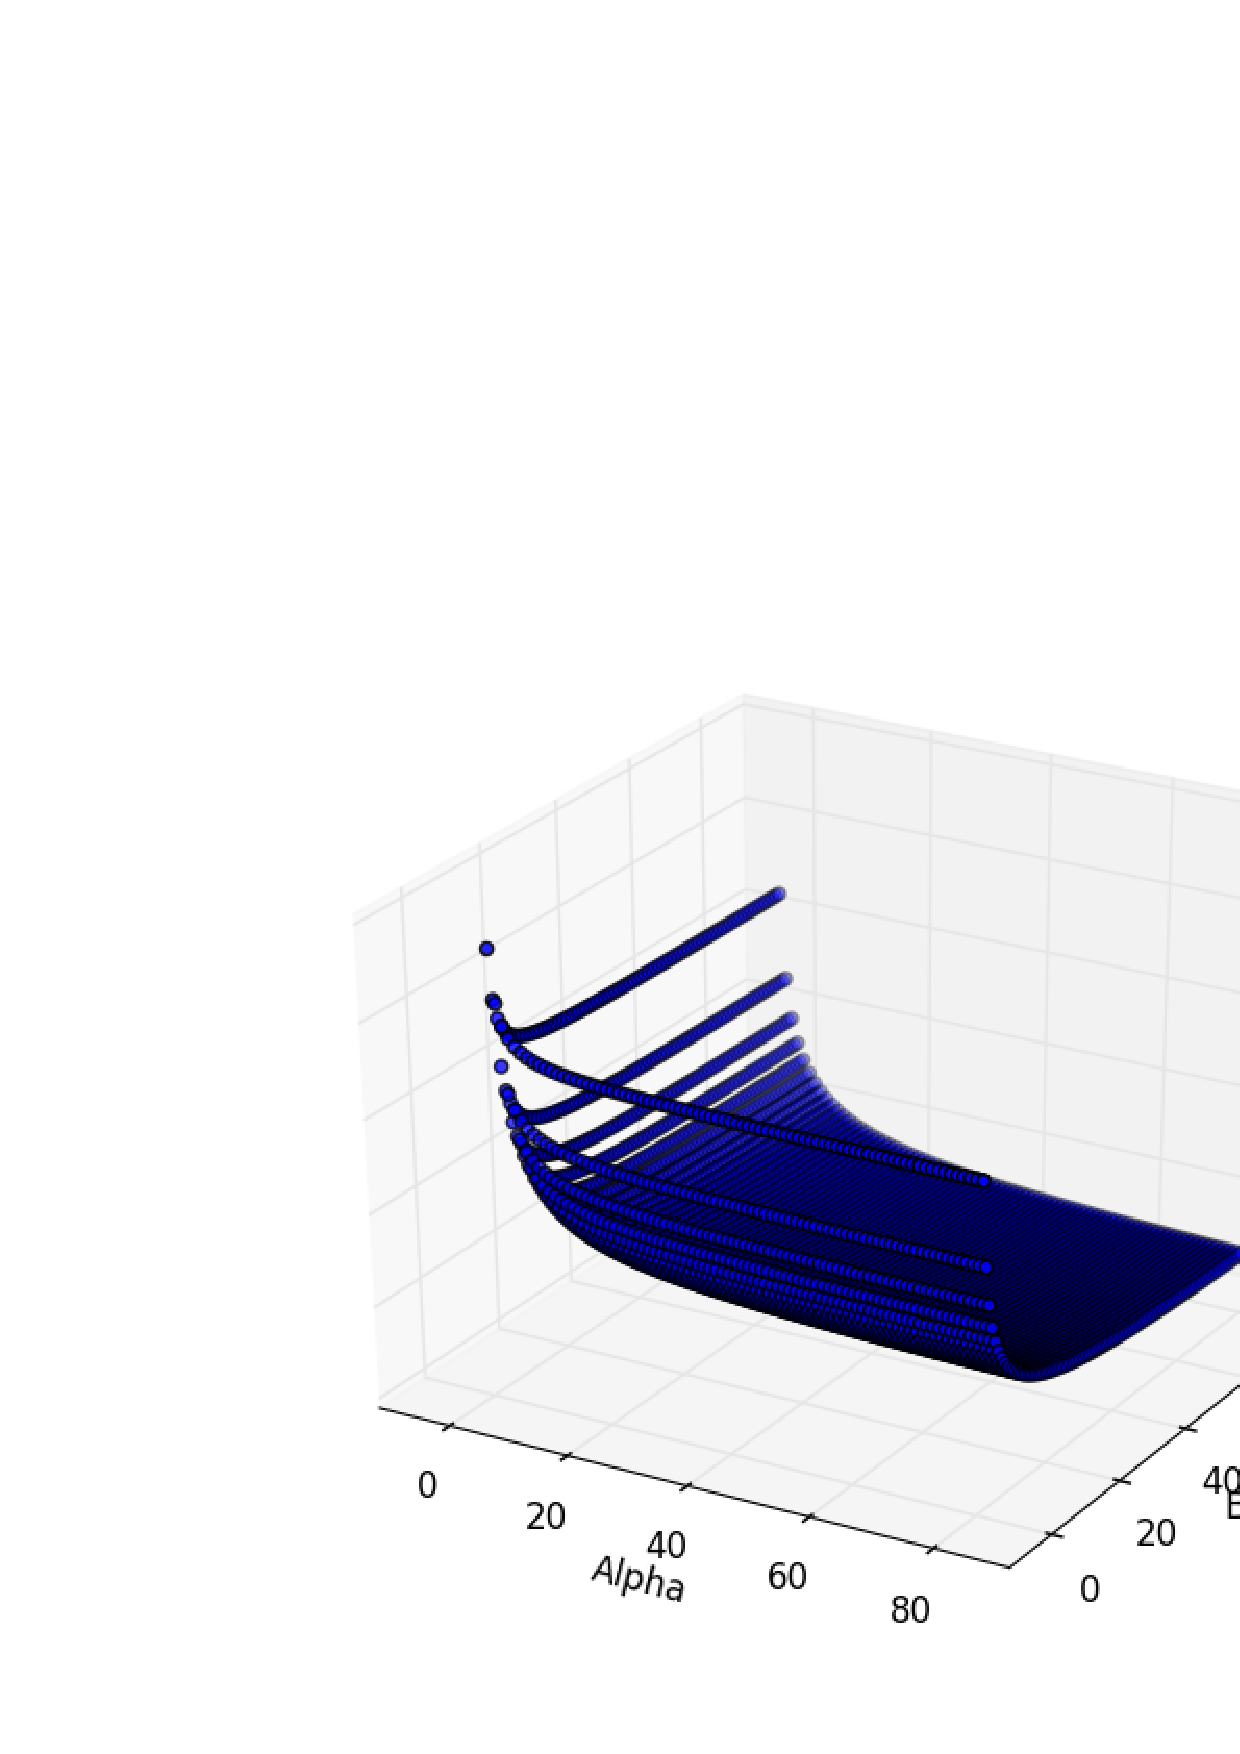
\includegraphics[width=0.48\textwidth]{sensitivity}
\caption{Hellinger distance study}
\label{fig_sensitivity}
\end{figure}
In this part, we firstly study the local sensitivity of Hellinger distance of different $\betad$ distributions as in Fig. \ref{fig_sensitivity}, in order to have a better understanding of the relationships between accuracy and next two aspects.


As in Fig. \ref{fig_sensitivity}, the local sensitivity of Hellinger distance will decrease when $\betad$ distribution's two parameters get closer (i.e. more uniform) and larger. In the same time, our smooth sensitivity will also decrease based on the Def. \ref{def_smoo}. From accuracy bound in Sec. \ref{subsec_accuracy_smoo}, the accuracy will be improved when sensitivity go larger. In consequence, when we increase the prior distribution, the smooth sensitivity in our exponential mechanism will decrease, which means our accuracy will be improved. However, the sensitivity of $l_1$ norm in Laplace mechanism is fixed regardless the prior distribution. We will study this trade-off in Sec. \ref{subsubsec_vs_prior}.

\subsubsection{Accuracy Analysis wrt. data variance}

Similar as above, when the data variance is small (i.e. the data are uniform), the parameters of posterior distribution will get more uniform (i.e. closer). Based on Fig. \ref{fig_sensitivity}, the Hellinger distance's sensitivity will get smaller when parameter get closer. As a result, the accuracy will be improved in the same time. We will study this trade-off in Sec. \ref{subsubsec_vs_variance}


\bibliographystyle{ACM-Reference-Format}
\bibliography{bayesian.bib}

\end{document}

